\part{Tools}

Um verlässliche Organisation und Kommunikation innerhalb des Teams zu gewährleisten, wurden verschiedene Tools benutzt.
Insbesondere sollte es einfach möglich sein, einen Überblick über den Status der Implementierung zu behalten.
Außerdem musste der durch die verwendeten Tools entstehende Mehraufwand minimal bleiben, um den zeitlichen Ansprüchen der Implementierung gerecht zu werden.
Folgende Tools wurden verwendet:

\section{Slack}

\begin{figure}[H]
\caption{Slack}
\centering
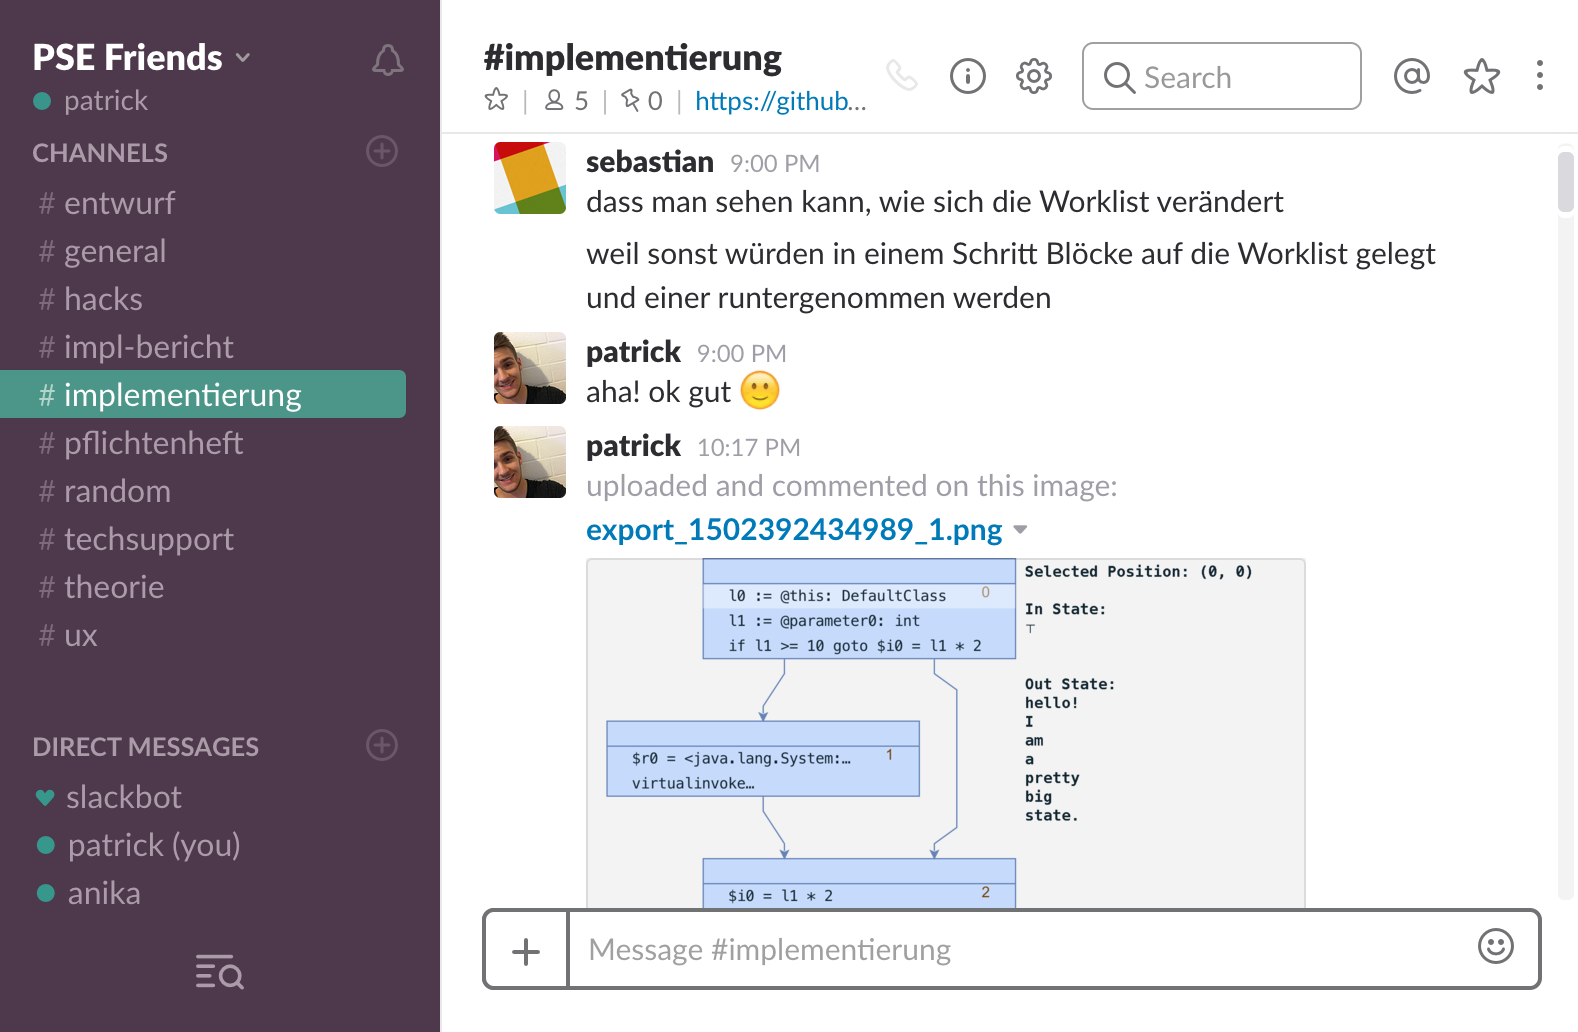
\includegraphics[width=0.8\textwidth]{slack.png}
\end{figure}

Slack ist ein Instant Messenger, der speziell auf Firmen und Teams ausgelegt ist.
Sowohl Kommunikation zwischen zwei als auch zwischen mehreren Personen ist möglich.
Darüber hinaus können Gruppen (Channels) erstellt werden, die sich einem bestimmten Thema widmen, z.B. \textit{Implementierung} oder \textit{Implementierungsbericht}, wodurch parallele Diskussionen ermöglicht werden.
Auch die Einbindung von Mediendateien ist einfach möglich.

Durch die Verwendung von Slack wurden Verzögerungen in der Kommunikation weitestgehend vermieden. 
Außerdem erwies es sich als geschicktes Tool, um Unklarheiten bezüglich der Implementierung direkt zu beseitigen und alle Teammitglieder auf den neuesten Stand zu bringen.

\newpage
\section{Trello}

\begin{figure}[H]
\caption{Trello}
\centering
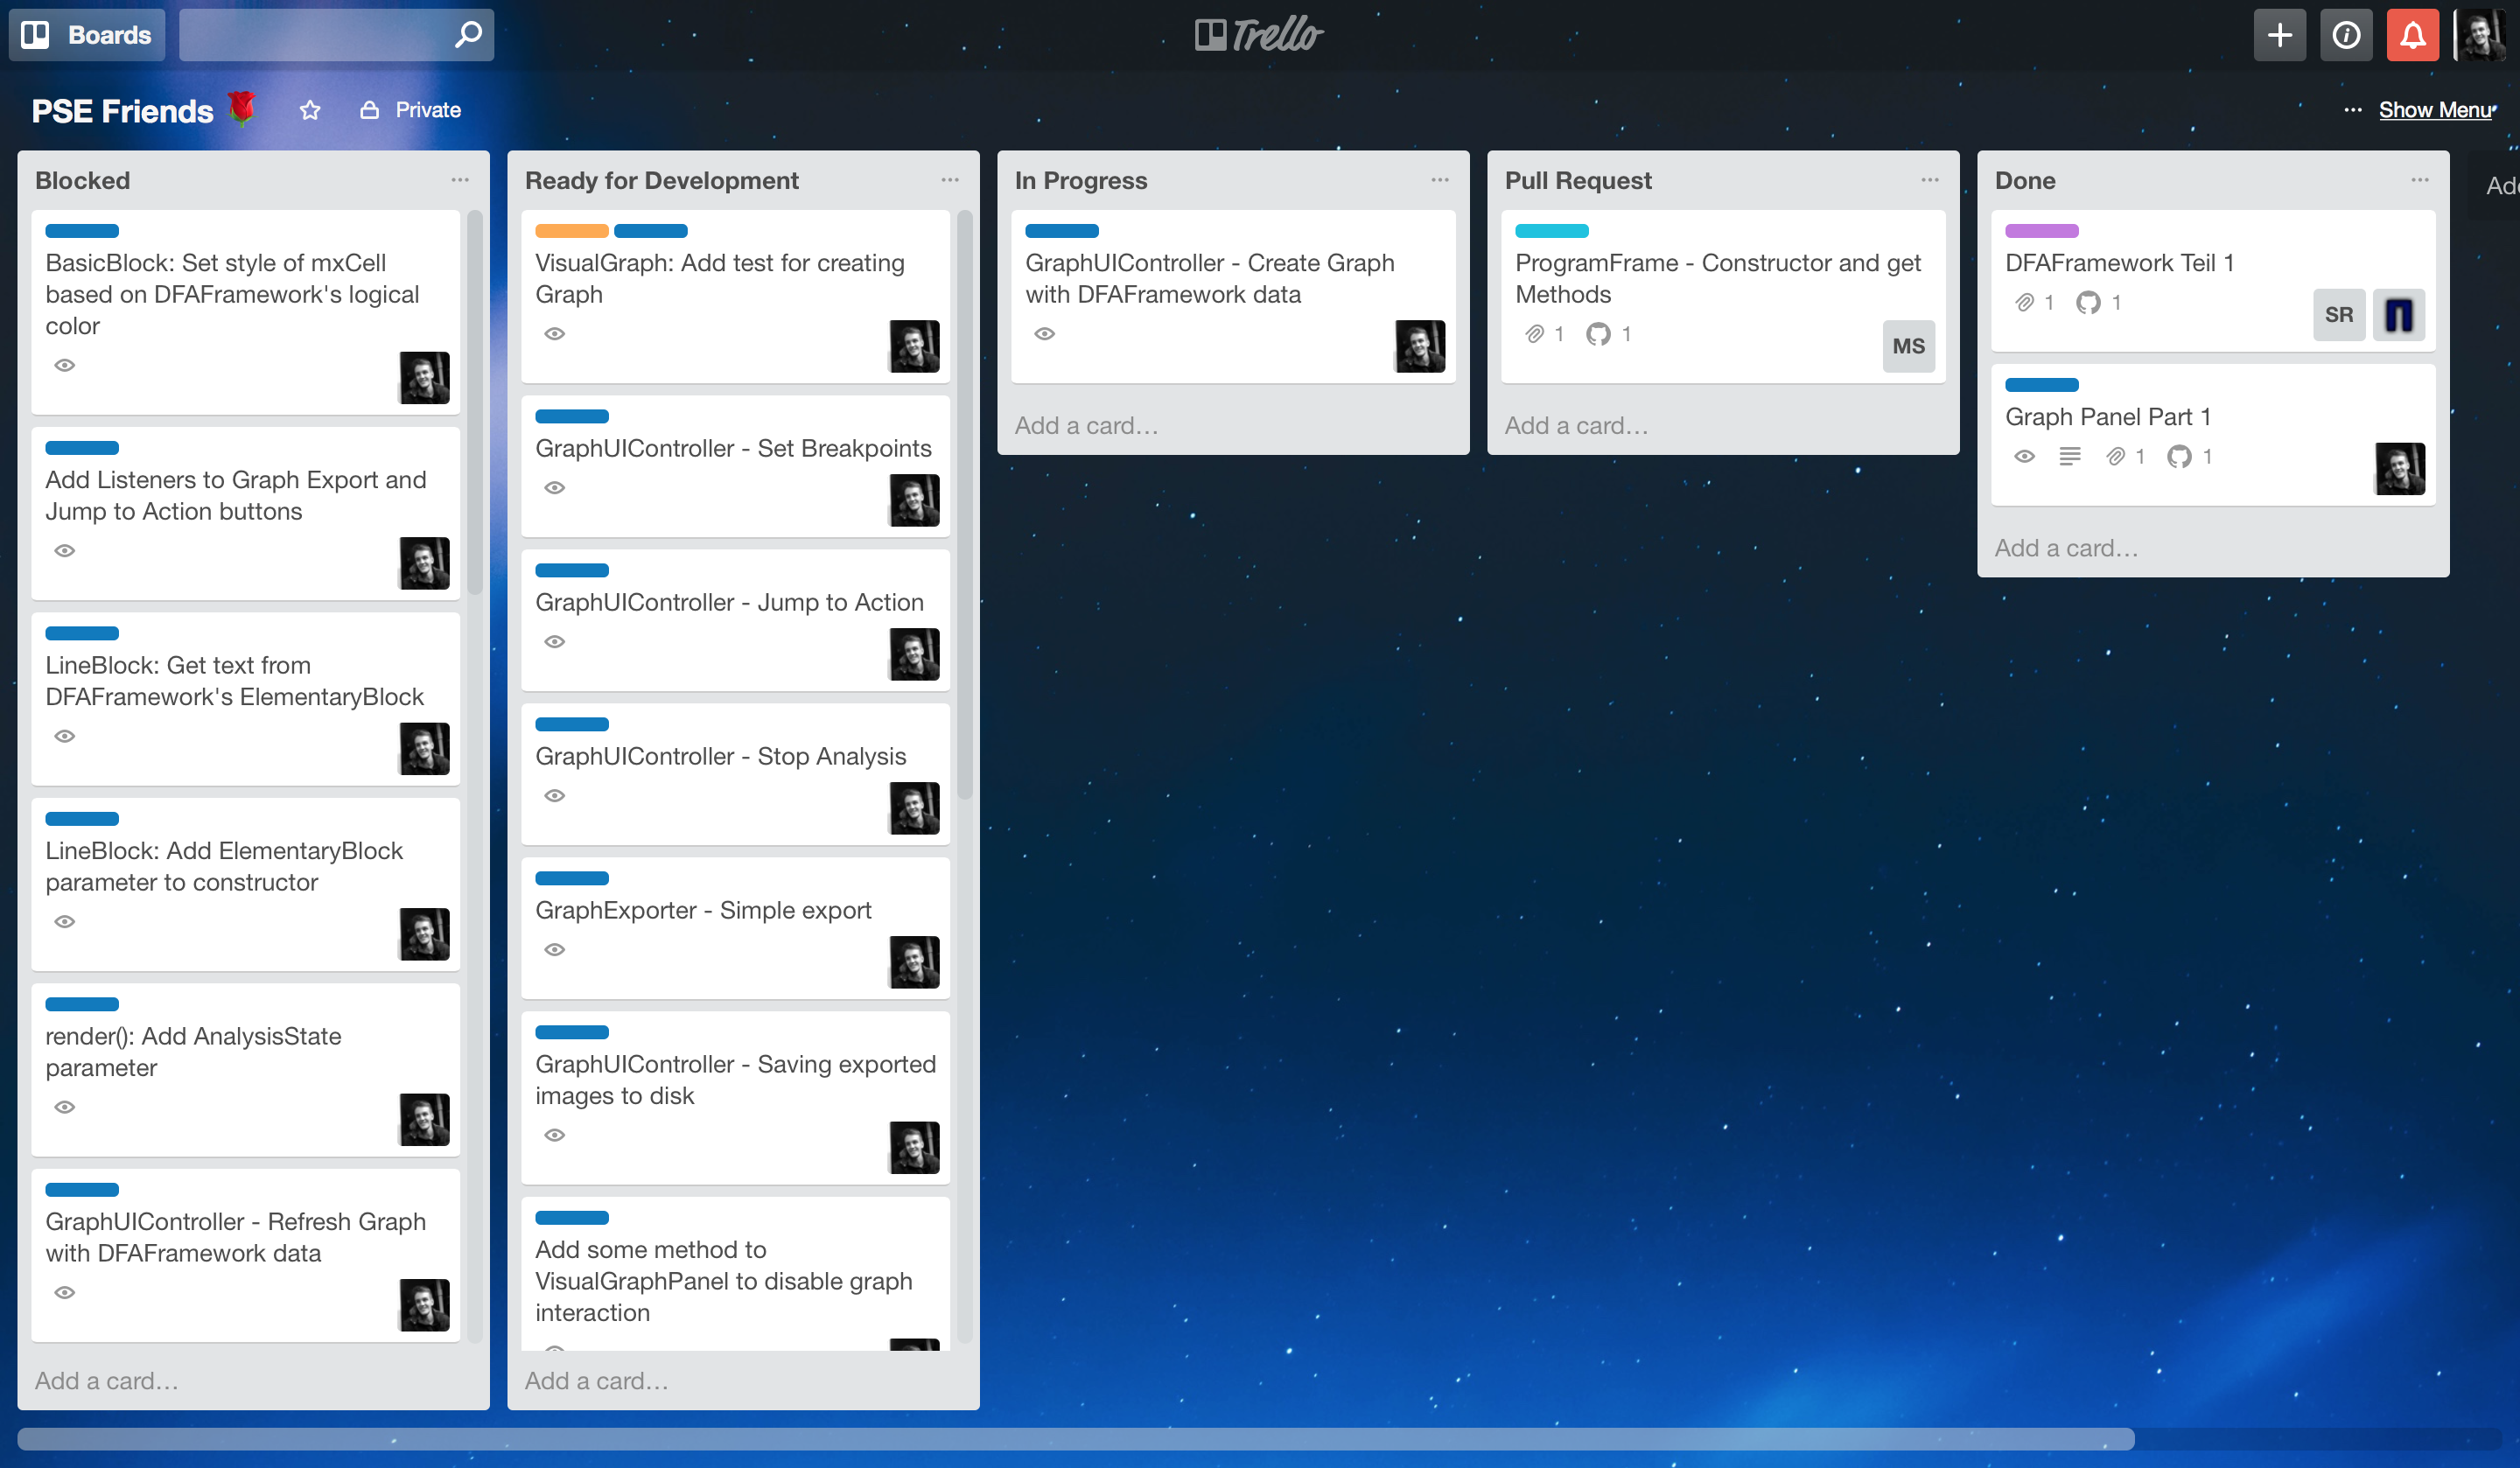
\includegraphics[width=0.8\textwidth]{trello.png}
\end{figure}

Trello ist ein Online-Task-Board, welches insbesondere von Teams genutzt werden kann.
Es ermöglicht, für jede anstehende Aufgabe eine virtuelle Karte zu erstellen, der eine oder mehrere Personen zugeordnet werden.
Je nach Status der Aufgabe kann die Karte dann in verschiedene Spalten verschoben werden.

Im Team wurden die fünf Spalten \textit{Blocked}, \textit{Ready for Development}, \textit{In Progress}, \textit{Pull Request} und \textit{Done} verwendet.
\textit{Blocked} steht hierbei für Aufgaben, die zum gegebenen Zeitpunkt noch durch Abhängigkeiten blockiert sind.

Die Nutzung von Trello ermöglichte es, einfach einen groben Überblick über den Stand der Implementierung zu behalten. 
Darüber hinaus konnten auch auftretende Fehler festgehalten werden.

\section{GitHub: Pull Requests und Code Reviews}

\begin{figure}[H]
\caption{Code Review in einem Pull Request auf GitHub}
\centering
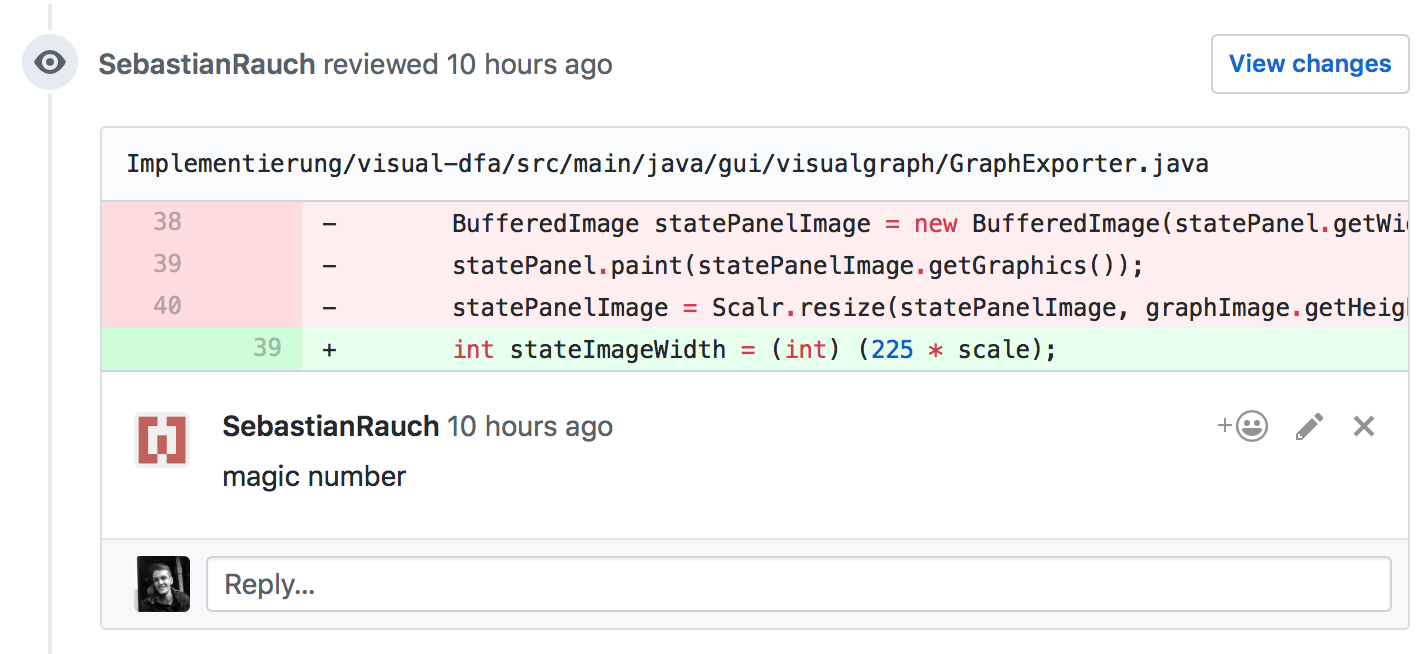
\includegraphics[width=0.8\textwidth]{github.png}
\end{figure}

Die für alle Phasen des Projekts genutzte Code-Plattform GitHub ermöglicht es, durch Pull Requests die Einführung von Änderungen zu strukturieren.
Im Team wurde festgelegt, dass vor Übernahme einer Änderung in den Hauptentwicklungszweig mindestens eine Person (nicht der Autor) diese überprüfen muss.

Das Ziel hierbei war die Identifizierung von Fehlern und Unklarheiten vor Übernahme in den Hauptentwicklungszweig.
Tatsächlich wurden einige häufig auftretende Fehlertypen (z.B. Off-By-One-Fehler) durch diese Vorgehensweise schnell aufgedeckt und behoben.
Darüber hinaus erwiesen sich Code Reviews als nützliche Hilfe, um allen Teammitgliedern eine aktuelle technische Übersicht des gesamten Programms zu bieten.

\newpage
\section{Jenkins}

\begin{figure}[H]
\caption{Ausschnitt einer Fehler-Nachricht wegen fehlgeschlagener Tests in Jenkins}
\centering
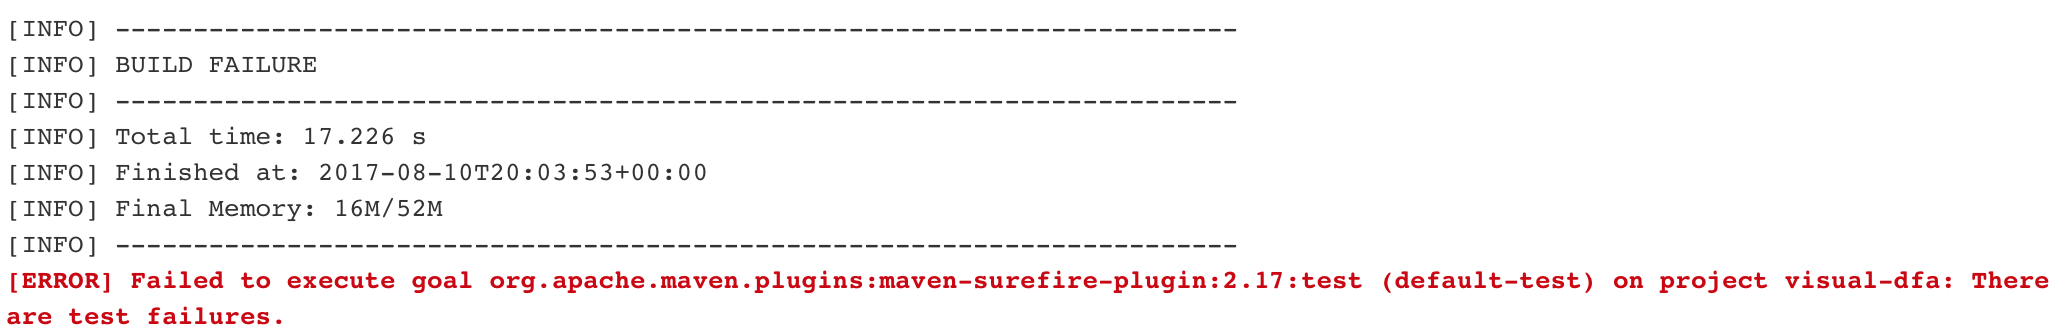
\includegraphics[width=0.8\textwidth]{jenkins.png}
\end{figure}

\begin{figure}[H]
\caption{Jenkins-Status in GitHub nach erfolgreichem Testdurchlauf}
\centering
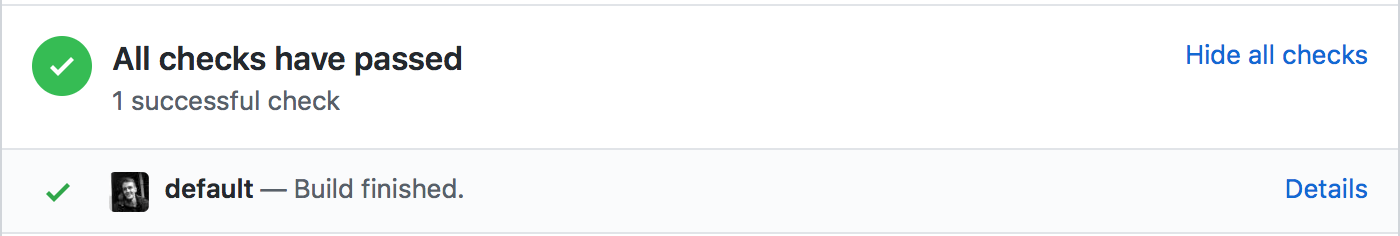
\includegraphics[width=0.8\textwidth]{jenkins-github.png}
\end{figure}

Jenkins ist ein webbasiertes Automatisierungs- und Integrationssystem, welches selbst gehostet werden kann. 

Um die Kompilierung des Programms und die Ausführung der JUnit-Tests bei jeder Änderung sicherzustellen, wurde dies automatisiert.
Dafür wurde mit Hilfe einer ec2-Instanz (Teil der Amazon Web Services) ein Server aufgesetzt, auf dem Jenkins installiert wurde.

Zusätzlich wurde eine Verbindung zu GitHub eingerichtet, sodass bei jeder Erstellung eines Pull Requests für alle Teammitglieder automatisch sichtbar war, ob der Testdurchlauf auf dem Server erfolgreich abgeschlossen wurde.

Trotz gelegentlich auftretender Probleme (Abstürze von Swing-Komponenten auf dem Server) erwies sich Jenkins als lohnenswerte zeitliche Investition und wird auch in der Qualitätssicherung Gebrauch finden.